\documentclass[]{article}
\usepackage[a4paper, total={15cm,23cm}]{geometry}
\usepackage{fancyhdr}
\usepackage{graphicx}
\usepackage{amsmath}
\usepackage{amssymb}
\usepackage{xcolor}
%opening
\title{PH 223 Week 1}
\author{Benjamin Bauml, Danielle Skinner, Grant Sherer}
\date{Winter 2024}
\pagestyle{fancy}
\rhead{PH 223}
\chead{Winter 2024}
\lhead{Week 1}

%Custom Quotation Command
\newcommand{\excerpt}[1]{\colorbox{lightgray}{\parbox{14.8cm}{#1}} \\}

\begin{document}

\maketitle

\begin{center}
Activity 1 is borrowed/adapted from Chapter 22 of \textit{Physics for Scientists and Engineers}.
\end{center}
\section*{Activity 1}%6
What mass of aluminum has a total nuclear charge of 1.0 C? Aluminum has atomic number 13 and molar mass 26.98 g/mol.
\iffalse
\excerpt{
What mass of aluminum has a total nuclear charge of 1.0 C? Aluminum has atomic number 13 and molar mass 26.98 g/mol.
}
% To reveal the solution, delete "\phantom{\parbox{\textwidth}{" from the beginning, and "}}" from the end.
\phantom{\parbox{\textwidth}{
Let $ N $ be the number of aluminum atoms, and let $ m $ be the mass we are looking for. It follows that the total charge $ Q = 13eN $ (where $ e = 1.60\times10^{-19} $ C is the charge on a single proton). We know that there are approximately $ 6.022\times10^{23} $ aluminum atoms in one mole of aluminum, and each mole has 0.02698 kg of mass. By using these ratios to convert units, we find
\[
\begin{split}
	m & = N \frac{1\text{ mol Al}}{6.022\times10^{23}\text{ Al atoms}} \frac{0.02698\text{ kg}}{1\text{ mo Al}} \\
	& = \frac{Q}{13e} \frac{0.02698\text{ kg}}{6.022\times10^{23}} \\
	& = \frac{1.0\text{ C}}{13(1.60\times10^{-19}\text{ C})} \frac{0.02698\text{ kg}}{6.022\times10^{23}} \\
	& \approx 2.15\times10^{-8}\text{ kg}.
\end{split}
\]
The mass of aluminum with the desired nuclear charge is 21.5 nkg, which is minuscule; this illustrates howw small atoms and protons are. Due to the equal number of electrons present, this chunk of aluminum would likely be close to neutral.
}}
\fi


%\pagebreak
%\section*{Activity 2}%10
%\excerpt{
%Two neutral metal spheres on wood stands are touching. A negatively charged rod is held directly above the top of the left sphere, not quite touching it. While the rod is there, the right sphere is moved so that the spheres no longer touch. Then the rod is withdrawn. Afterward, what is the charge state of each sphere? Use charge diagrams to explain your answer.
%}
% To reveal the solution, delete "\phantom{\parbox{\textwidth}{" from the beginning, and "}}" from the end.
%\phantom{\parbox{\textwidth}{
%\begin{center}
%	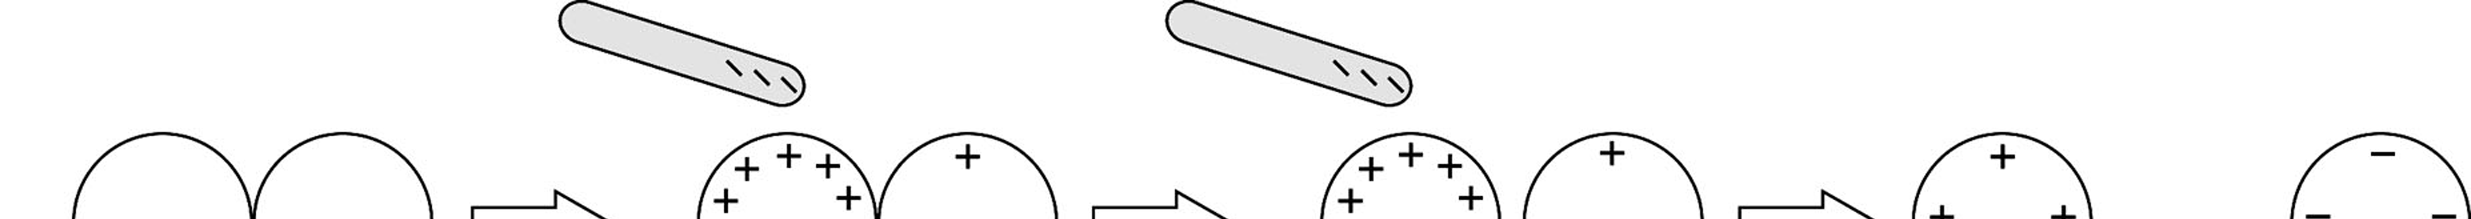
\includegraphics[scale=0.1]{SpheryHorror}\vspace{-0.5pt}
%	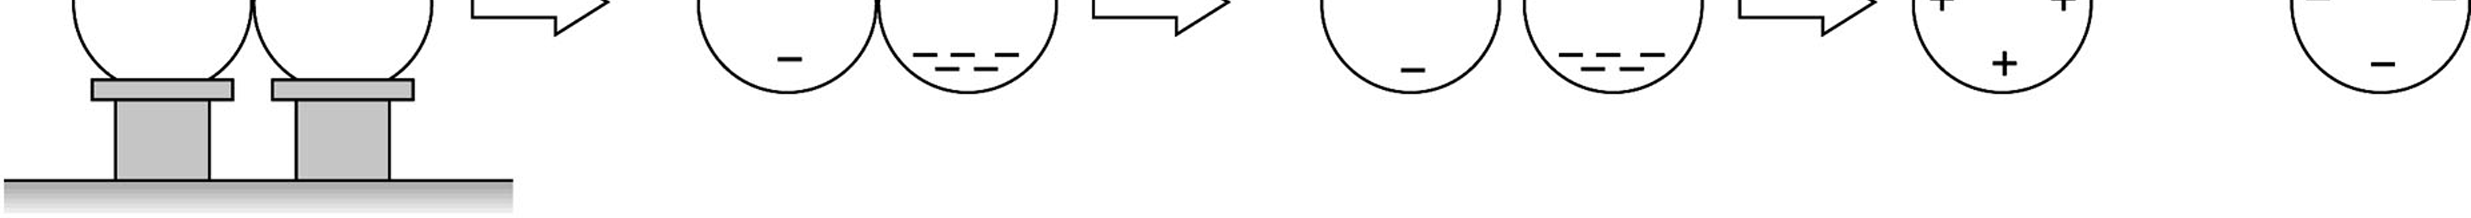
\includegraphics[scale=0.1]{SpheryHorrorLowerHalf}
%\end{center}
%\begin{itemize}
%	\item The first step shows two neutral metal spheres touching each other.
%	\item In the second step, the negative rod repels the negative charges, which will retreat as far as possible from the top of the left sphere. Note that the two spheres are touching and the net charge on these two spheres is still zero.
%\end{itemize}
%}}
%\pagebreak%Uncomment when revealing solutions.
%\phantom{\parbox{\textwidth}{
%\begin{itemize}
%	\item While the rod is there on top of the left sphere, the right sphere is moved away from the left sphere. Because the right sphere has an excess negative charge, charge conservation implies the left sphere must have the same magnitude of positive charge. Upon separation, the negative charge is trapped on the right sphere, as shown in the third step.
%	\item As the two spheres are moved farther apart and the negative charged rod is moved away from the spheres, the charges on the two spheres redistribute uniformly over the entire surface of each sphere. Thus, we are left with two oppositely charged spheres.
%\end{itemize}
%}}

\iffalse
%\pagebreak
\section*{Activity 3}
\excerpt{
(a) To derive Kepler's 3rd law, one can start by equating the gravitational force and the centripetal force necessary for uniform circular motion:
\[
F_{g} = \frac{GMm}{r^{2}} = \frac{4\pi^{2}mr}{T^{2}} = F_{c},
\]
where we have made use of the substitution $ \omega = 2\pi f = \frac{2\pi}{T} $. Let us model protons and electrons as classical point particles, with the electron in uniform circular motion around the proton. How would we change the above condition to account for the effects of charge?
}
% To reveal the solution, delete "\phantom{\parbox{\textwidth}{" from the beginning, and "}}" from the end.
\phantom{\parbox{\textwidth}{
To account for the Coulomb interaction, we need to insert a term of the form
\[
\frac{Kq_{1}q_{2}}{r^{2}}.
\]
The charge on an electron is $ -e $, and the charge on a proton is $ +e $, which would make the force between the two particles attractive. As such, the magnitude of the Coulomb force between a proton and an electron (which is $ \frac{Ke^{2}}{r^{2}} $) adds to the attractive gravitational force to create the net centripetal force. Our equation should be
\[
\frac{GMm}{r^{2}} + \frac{Ke^{2}}{r^{2}} = \frac{4\pi^{2}mr}{T^{2}}.
\]
}}
\excerpt{
(b) Let $ e = 1.60\times10^{-19} $ C be the magnitude of charge on a proton or electron, $ M = 1.67\times10^{-27} $ kg be the mass of the proton, and $ m = 9.11\times10^{-31} $ kg be the mass of an electron. Compare $ GMm $ and $ Ke^{2} $ in terms of order of magnitude (the powers of 10 in scientific notation). Are they similar, or is one much larger than the other?
}
% To reveal the solution, delete "\phantom{\parbox{\textwidth}{" from the beginning, and "}}" from the end.
\phantom{\parbox{\textwidth}{
Considering only orders of magnitude, $ G \sim 10^{-11} $ Nm$ ^{2}/ $kg$ ^{2} $, $ M \sim 10^{-27} $ kg, and $ m \sim 10^{-30} $ kg (because the leading 9 in $ 9.11\times10^{-31} $ is close to another order of magnitude). As such, $ GMm \sim 10^{-68} $ Nm$ ^{2} $. For the electric terms, $ K \sim 10^{10} $ Nm$ ^{2}/ $C$ ^{2} $ (because the leading 9 in $ 9\times10^{9} $ is close to another order of magnitude) and $ e \sim 10^{-19} $ C. Thus, $ Ke^{2} \sim 10^{-28} $ Nm$ ^{2} $. Clearly, $ GMm \ll Ke^{2} $ (by about 40 orders of magnitude). For those who want an exact calculation:
\[
\begin{split}
	GMm & = (6.67\times10^{-11}\text{ Nm}^{2}/\text{kg}^{2})(1.67\times10^{-27}\text{ kg})(9.11\times10^{-31}\text{ kg}) = 1.01\times10^{-67} \text{ Nm}^{2}; \\
	Ke^{2} & = (9\times10^{9}\text{ Nm}^{2}/\text{C}^{2})(1.60\times10^{-19}\text{ C})^{2} = 2.30\times10^{-28}\text{ Nm}^{2}.
\end{split}
\]
We were off by an order of magnitude in the first expression, because $ 6.67\times1.67 = 11.1389 \sim 10 $. Still, $ GMn \ll Ke^{2} $ (by 39 orders of magnitude). We can safely ignore the contribution of the gravitational force to this situation.
}}
\pagebreak \\
\excerpt{
(c) Take your modified expression from part (a) and remove the gravitational term. If we take the distance between the proton and the electron to be $ r = 5.29\times10^{-11} $ m (the Bohr radius), then what order of magnitude is the rotational frequency of the electron? What SI prefix should I be appending to hertz when I express this frequency?
}
% To reveal the solution, delete "\phantom{\parbox{\textwidth}{" from the beginning, and "}}" from the end.
\phantom{\parbox{\textwidth}{
Without the gravitational term, our expression becomes
\[
\frac{Ke^{2}}{r^{2}} = \frac{4\pi^{2}mr}{T^{2}} = 4\pi^{2}mrf^{2}.
\]
Solving for frequency, we find
\[
f = \sqrt{\frac{Ke^{2}}{4\pi^{2}mr^{3}}}.
\]
We already know that $ Ke^{2} \sim 10^{-28} $ Nm$ ^{2} $ and $ m \sim 10^{-30} $ kg. Furthermore, $ \pi^{2} \sim 10 $, and because $ 5^{3} = 125 $, we should be choose $ r^{3} \sim 10^{-31} $ instead of $ 10^{-33} $. Finally, let us consider 4 to be on the order of 1. All together, this means
\[
\frac{Ke^{2}}{4\pi^{2}mr^{3}} \sim \frac{10^{-28}\text{ Nm}^{2}}{10\times10^{-30}\times10^{-31}\text{ kg m}^{3}} = 10^{32}\text{ s}^{-2}.
\]
Thus $ f \sim 10^{16} $ Hz, which would be on the order of ten petahertz. An exact calculation shows
\[
f = \sqrt{\frac{2.30\times10^{-28}\text{ Nm}^{2}}{4\pi^{2}(9.11\times10^{-31}\text{ kg})(5.29\times10^{-11}\text{ m})^{3}}} \approx \sqrt{4.32\times10^{31}\text{ s}^{-2}} \approx 6.57\times10^{15}\text{ Hz}
\]
We were off by one order of magnitude for discounting the full effect of certain minute details. The frequency is on the order of one petahertz.
}}
\fi

\section*{Activity 2}%6
You dip a candy bar into chocolate and pull it out slowly so that more and more chocolate accu- mulates on the bar. When the chocolate has cooled, you measure the mass density at one end to be $\lambda = 0$ and the density at the other end to be $\lambda = \alpha L$, where L is the length of the bar and $\alpha$ is a constant, and you assume the mass density is linearly proportional to distance along the candy bar.
\begin{enumerate}
	\item How are $\lambda$, mass, and length related?
	\item Can you represent this relationship as a derivative?
	\item Determine the total mass of chocolate on the candy bar.
	\item The expression for center of mass is 
	\begin{equation}
		x_{cm} = \frac{1}{m_i}\int_{x_i}^{x_f} x dm
	\end{equation}
	Use this expression to find the center of mass of the chocolate bar.
\end{enumerate}
\iffalse
\excerpt{You dip a candy bar into chocolate and pull it out slowly so that more and more chocolate accu- mulates on the bar. When the chocolate has cooled, you measure the mass density at one end to be $\lambda = 0$ and the density at the other end to be $\lambda = \alpha L$, where L is the length of the bar and $\alpha$ is a constant, and you assume the mass density is linearly proportional to distance along the candy bar.}
\vspace{50mm}
\excerpt{(a) How are $\lambda$, mass, and length related?}
\vspace{50mm}
% To reveal the solution, delete "\phantom{\parbox{\textwidth}{" from the beginning, and "}}" from the end.
\phantom{\parbox{\textwidth}{}}
\excerpt{(b) Can you represent this relationship as a derivative?}
\vspace{50mm}
\phantom{\parbox{\textwidth}{}}
\excerpt{(c) Determine the total mass of chocolate on the candy bar.}
\vspace{50mm}
\phantom{\parbox{\textwidth}{}}
\excerpt{(d) The expression for center of mass is 
\begin{equation}
	x_{cm} = \frac{1}{m_i}\int_{x_i}^{x_f} x dm
\end{equation}
Use this expression to find the center of mass of the chocolate bar.
}
\phantom{\parbox{\textwidth}{}}
\fi

\section*{Activity 3}%6
For each of the following charge density distributions, determine the units of the constant of proportionality ($\alpha, \beta, \gamma$) and the total charge:
\begin{enumerate}
	\item A rod of length $L$ oriented along the x-axis with charge distribution $\lambda (x) = \alpha x^{1/3}$.
	\item A rod of length $L$ oriented along the y-axis with charge distribution $\lambda (y) = \beta y^{5}$
	\item A disk of radius $R$ with charge distribution $\sigma (x,y) = \gamma xy$
\end{enumerate}
\iffalse
\excerpt{For each of the following charge density distributions, determine the units of the constant of proportionality ($\alpha, \beta, \gamma$) and the total charge:
\begin{enumerate}
	\item A rod of length $L$ oriented along the x-axis with charge distribution $\lambda (x) = \alpha x^{1/3}$.
	\item A rod of length $L$ oriented along the y-axis with charge distribution $\lambda (y) = \beta y^{5}$
	\item A disk of radius $R$ with charge distribution $\sigma (x,y) = \gamma xy$
\end{enumerate}}
\fi

\end{document}
